%%---------------------------------------------------------------------
%	Preamble
%	AMS gruppe 12
%	AMS F18
%---------------------------------------------------------------------
\documentclass[12pt,fleqn,a4paper]{article}
\usepackage[utf8]{inputenc}
\usepackage[danish]{babel}
\usepackage[top=2.5cm, left=2cm, right=2cm, bottom=2.5cm]{geometry}
\usepackage{graphicx}
\usepackage[bottom]{footmisc}
\usepackage{framed}
\usepackage{caption}
\usepackage{float}
\usepackage{mdframed}
\usepackage{listings}
\usepackage{color}
\usepackage[T1]{fontenc}
\usepackage{amsmath,amsfonts,amsthm} % Math packages
\usepackage{array}
\usepackage{wrapfig}
\usepackage{multirow}
\usepackage{tabu}
\usepackage{longtable}
\usepackage{lastpage}
\usepackage{fancyhdr}
\usepackage[compact]{titlesec}
\usepackage[table,xcdraw]{xcolor}
\usepackage{arydshln}
\usepackage[isbn,issn,url]{dk-bib}
\usepackage[toc,page]{appendix}
\usepackage{url}
\def\UrlBreaks{\do\/\do-}

\definecolor{mygreen}{RGB}{28,172,0} % color values Red, Green, Blue
\definecolor{mylilas}{RGB}{170,55,241}
\renewcommand{\lstlistingname}{Kodeudsnit}
\tabulinesep=3mm

\setcounter{secnumdepth}{2}
\setcounter{tocdepth}{2}

\setlength{\parindent}{0mm} %intet indryk
\setlength{\parskip}{3mm} 	%linjeskift v. afsnit

% Ændring af enumerize og itemize 
\usepackage{enumitem} % @http://ctan.org/pkg/enumitem
\setlist[itemize]{topsep=0pt, itemsep=0.5pt}
\setlist[enumerate]{topsep=0pt, itemsep=0.5pt}

%afstand omkring sections
\titlespacing{\section}{0pt}{5mm}{0pt}
\titlespacing{\subsection}{0pt}{2mm}{0pt}
\titlespacing{\subsubsection}{0pt}{2mm}{0pt}

\usepackage{arydshln}
%aryd
\setlength\dashlinedash{3pt}
\setlength\dashlinegap{4pt}

\lstset{language=C++,
	breaklines=true,
	keywordstyle=\color{blue},
	stringstyle=\color{red},
	commentstyle=\color{mygreen},
	morecomment=[l][\color{magenta}]{\#}
}

%header & footer
\makeatletter
\pagestyle{fancy}
\fancypagestyle{plain}{}
\renewcommand{\chaptermark}[1]{\markboth{#1}{}}
\setlength{\headheight}{35pt}
\fancyfoot{} % clear all fields
\fancyfoot[R]{Side \thepage\ af \pageref{LastPage}}
\fancyhead{} % clear all fields
\fancyhead[L]{
\includegraphics[clip, trim = 0 0 240pt 0, height=30pt]{Figur/IHA_AU_logo.png}}
\fancyhead[R]{Forår 2018}
\fancyhead[C]{Anvendte Microcontroller Systemer}
\renewcommand{\headrulewidth}{0pt}

\def\thickhrulefill{\leavevmode \leaders \hrule height 1.2ex \hfill \kern \z@}
\def\@makechapterhead#1{
  \vspace*{10\p@}%
  {\parindent \z@ \centering \reset@font
        \thickhrulefill\quad 
        \scshape\bfseries\textit{\@chapapp{}  \thechapter}  
        \quad \thickhrulefill
        \par\nobreak
        \vspace*{10\p@}%
        \interlinepenalty\@M
        \hrule
        \vspace*{10\p@}%
        \Huge \bfseries #1 \par\nobreak
        \par
        \vspace*{10\p@}%
        \hrule
        \vskip 40\p@
  }}

\usepackage{tcolorbox}
\definecolor{mycolor}{rgb}{0.122, 0.435, 0.698}% Rule colour
\makeatletter
\newcommand{\mybox}[1]{%
	\setbox0=\hbox{#1}%
	\setlength{\@tempdima}{\dimexpr\wd0+13pt}%
	\begin{tcolorbox}[colframe=mycolor,boxrule=0.5pt,arc=4pt,
		left=6pt,right=6pt,top=6pt,bottom=6pt,boxsep=0pt]
		#1
	\end{tcolorbox}
}
\makeatother

\graphicspath{ {Figur/} }


%Se Kodeudsnit \ref{lstlisting:generel_kode}

%\captionof{lstlisting}{Generelle egenskaber for koden til fremstilling af diverse figure i matlab} 
%\label{lstlisting:generel_kode}
%\vspace{5mm} %5mm vertical space
%
%\subsection{Kode til lyd i forhold til tiden}
%\begin{framed}
%\begin{center}
%\begin{lstlisting}
%figure('name','trafikstoejen i fuld laengde'); clf
%subplot(211);
%plot(t,s_sound_left)
%xlabel('Tid (sek)')
%ylabel('Signalstyrke')
%title('Trafikstoej set i forhold til tiden')
%grid on
%hold on
%\end{lstlisting}
%\end{center}
%\end{framed}




%\begin{document}

\section{Wifi-klassen}
Wifi-klassens ansvar er at oprette en TCP-forbindelse mellem PC'en og Kontrolenheden, samt sende og modtage beskeder over denne forbindelse.

Til at oprette TCP-forbindelsen anvendes en TCP-socket, der sørger for at påsætte TCP-headeren og overholde TCP-protokollens validering. 
For at simplificere interfacet med socketen, implementeres oprettelse og nedlæggelse af socketen i Wifi-klassen. 
Derudover sørger Wifi-klassen for at der ikke opstår timing problemer i kommunikationen.  \\
Wifi-klassen designes således, at den kan anvendes på både PC’en og Kontrolenheden med hver sin 'opret forbindelse' funktion. 
Kontrolenheden designes som server for TCP-forbindelsen og PC’en som klient.
Forbindelses funktionerne er implementeret i Wifi-klassens \textit{connectToPc()} og \textit{connectToRobot()}.
Oprettelsen af TCP-forbindelsen kan ses på figur \ref{fig:wifi_connect_tcp}.

\begin{figure} [H]
\centering
	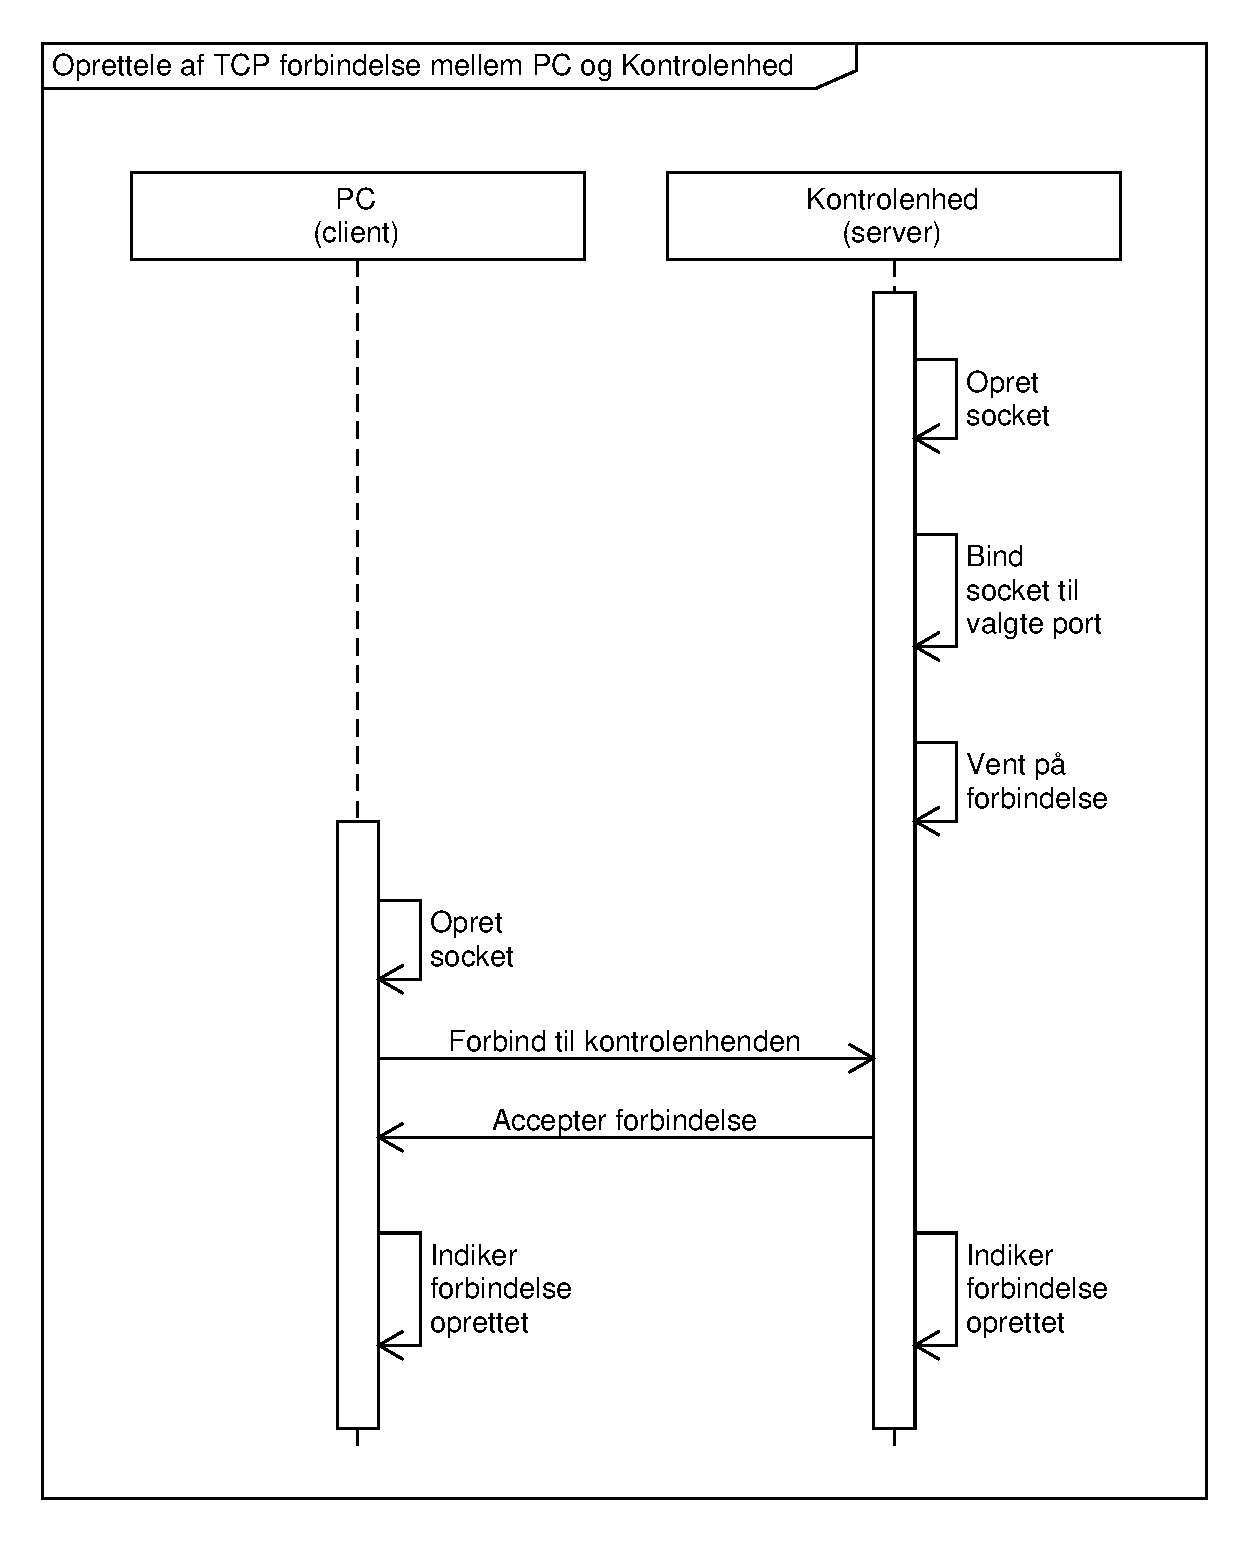
\includegraphics[width=0.55 \textwidth]{wifi_connect_tcp.pdf}
	\captionof{figure}{Oprettelse af TCP-forbindelsen mellem PC og Kontrolenhed}
	\label{fig:wifi_connect_tcp}
\end{figure}

I Wifi-klassen findes også funktionerne \textit{sendCmd()} og \textit{readCmd()}, der henholdsvis sender og modtager en besked til TCP-socketen. \\
Da socketen er full-duplex, kan der både skrives til og læses fra socketen på samme tid. 
Det er dog ikke tilladt at skrive til socketen fra flere steder samtidigt.
Det samme gælder for læsning.
Dette sikres i praksis med en mutex, der skal tages før en tråd får rettighed til at sende. Der er en tilsvarende mutex til læsning. \\
Derudover sikres det, at socketen ikke anvendes før det indikeres, at forbindelsen er oprettet.
Dette sker ved brug af et betinget signal, som ventes på indtil der er oprettet forbindelse.


\subsection{Enhedstest}
For at teste Wifi-klassen anvendes to virtuelle maskiner, én til PC og én til Kontrolenheden, med en forbindelse, der simulerer Wifi-forbindelsen. 
Til testen opsættes tre test cases, som skal gennemføres før klassen kan godkendes, disse er som følgende:
	
	\begin{enumerate}
	\item Skal kunne oprette en TCP-forbindelse mellem to maskiner.
	\item Skal kunne sende en besked fra en maskine som kan læses på den anden.
	\item Socketen må ikke tilgås før der er oprettet forbindelse.
	\end{enumerate}
	
For udførsel af testen se bilag \ref{appendix:BilagEnhedstestWifi}.

Efter testen kan det konkluderes, at Wifi-klassen opfylder sit ansvar og er sikret mod timing problemer.

%\end{document}